\section{Community dynamics of question answering}
Except answering to a proposed question, voting is another significant mechanism in Stack Overflow. Community users can evaluate the quality or usefulness of an answer by giving them a vote up or vote down. In this section, we focus on both investigate answering and voting mechanisms. Specifically, we want to find out how answerers' reputation correlates to the answers' arrival time. In addition, different scenarios from various questions' activeness are also our concern. To investigate these concerns, we reveal underlying scenarios behind Stack Overflow community, the result can be useful for researchers to possess a deeper understanding and insights on Stack Overflow. 

\subsection{A reputation pyramid}
A reputation mechanism adopted in Stack Overflow, it can be accumulate by answering questions, collecting more vote scores or winning a bonus. Usually, reputation is a significant standard to evaluate an answerer's expertness. In Stack Overflow, answerers are encouraged to answer a question quickly. In this scenario, we would expect an answerer with high reputation to be the provide timely correct answers. 

%Fig 1
\begin{figure}[!t]
    \centering
    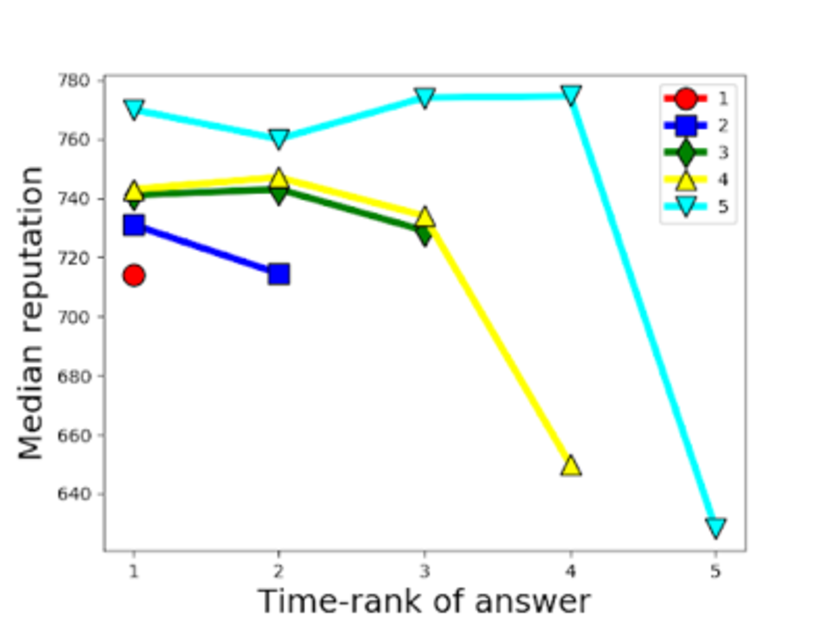
\includegraphics[width=0.7\columnwidth]{img/Fig1_2010.pdf}
    \caption{Median reputation versus answer time-rank. Questions with a total of 1 to 5 answers plotted (one curve each). High reputation users tend to answer early. (From 2008/07/31 to 2010/12/31)}
    \label{fig:fig1_2010}
\end{figure}

\begin{figure}[!t]
    \centering
    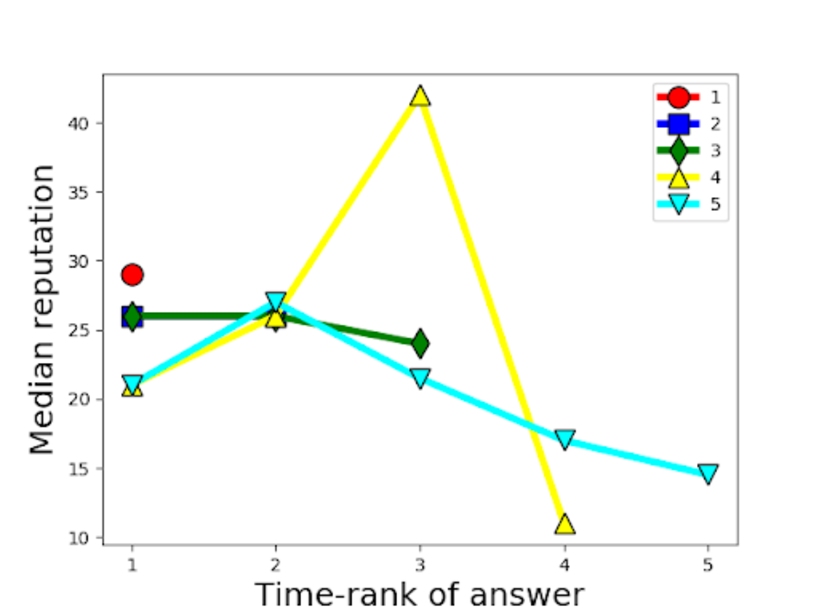
\includegraphics[width=0.7\columnwidth]{img/Fig1_2017.pdf}
    \caption{Median reputation versus answer time-rank. Questions with a total of 1 to 5 answers plotted (one curve each). High reputation users tend to answer early. (From 2015/07/31 to 2017/12/31)}
    \label{fig:fig1_2010}
\end{figure}

From Fig \ref{fig:fig1_2010} we calculate the median reputation of different answerers in a time-rank sequence, which means the answers of a question arrive successively. We find in most cases, the early answerers in the time-rank sequence usually have a relatively high reputation, and the later answerers are inclined to have lower reputations. This decrease is especially obvious when analyzing low speed answerers' reputation. The fact indicates that answerers' reputation can be utilized in evaluating whether if a question has been sufficiently answered, this will serve as the foundation of following prediction work.


\subsection{The activity level of a question}
In the previous section, we illustrate the structure of users' reputation pyramid, which explains how answers arrival process relates to the user's reputation, as well as other phenomena from our observation. In this section, we would investigate more on voting, another significant mechanism of Stack Overflow. Except for merely answerers and questioners, other users can also involve in those QA sections by commenting, voting, etc.. The voting mechanism is not only applicable to answers but also to questions, and it is also considered as an important factor to reflect community involvement and evaluation. From our observation of Stack Overflow, we notice that questions with more answers are more likely to benefit from community involvement: answers will get higher votes and questions will receive more favorites. Highly active QA processes are more inclined to benefit from the community, instead of a competence among answerers themselves.  Based on our observation, our goal is to validate whether if the activity level is able to explain the feedback and evaluation from the community activities.

\textbf{Higher activity produces benefits.}
Like we discussed, unlike the features of general QA sites, Stack Overflow is programming-oriented, the questions are generally hard to be answered by majority community users. Furthermore, based on our observation from the previous section, answerers' arrival time is related to acceptance rate and answerers' reputation, it motivates answerers to answer a question quickly once it is posted. However, is there a competitive relationship existing among answerers?

%Fig6
%2010
\begin{figure}[!t]
    \centering
    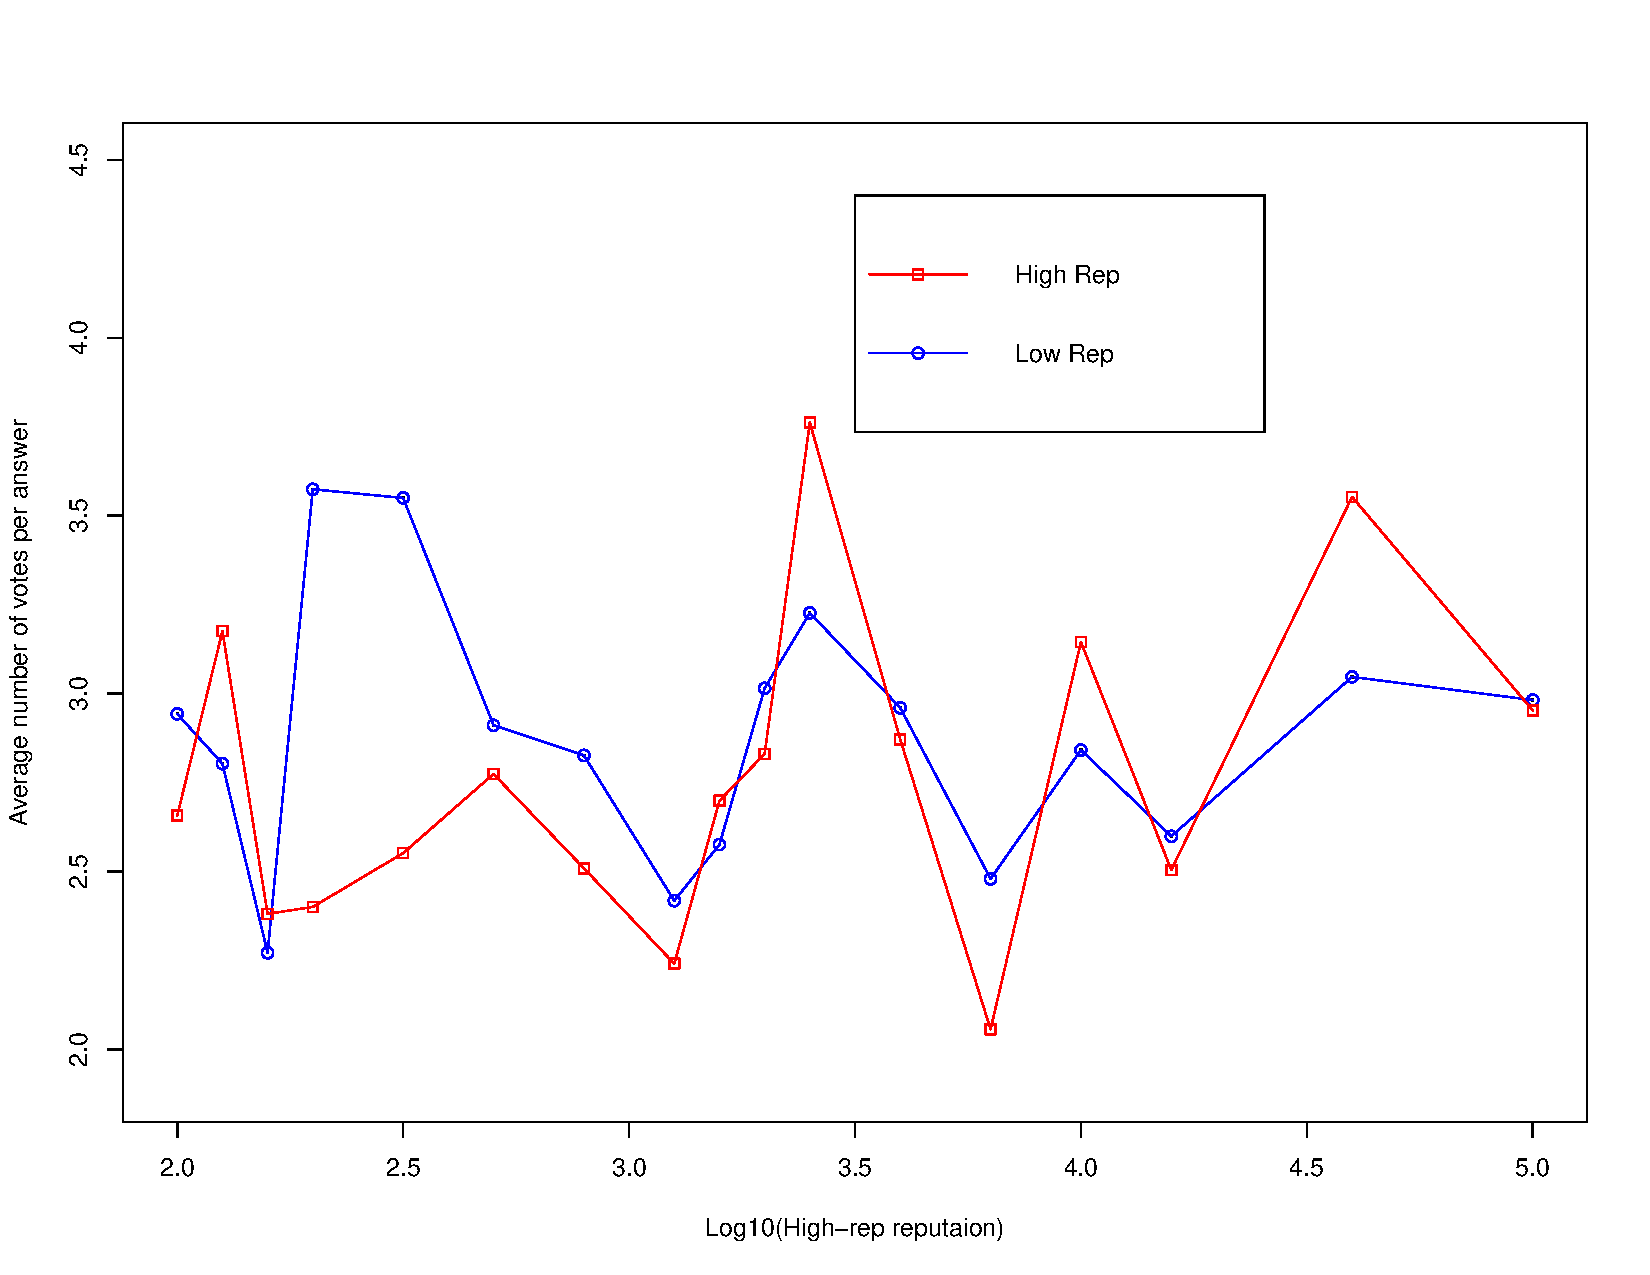
\includegraphics[width=0.8\columnwidth]{img/Fig6_2010.pdf}
    \caption{Average number of votes per answer for both answerers on a 2-answer question as a function of the higher answerer reputation. Lower reputation fixed between 75-125. High reputation plotted on a logarithmic (base 10) scale. (From 2008/07/31 to 2010/12/31)}
    \label{fig:fig6_2010}
\end{figure}

\begin{figure}[!t]
    \centering
    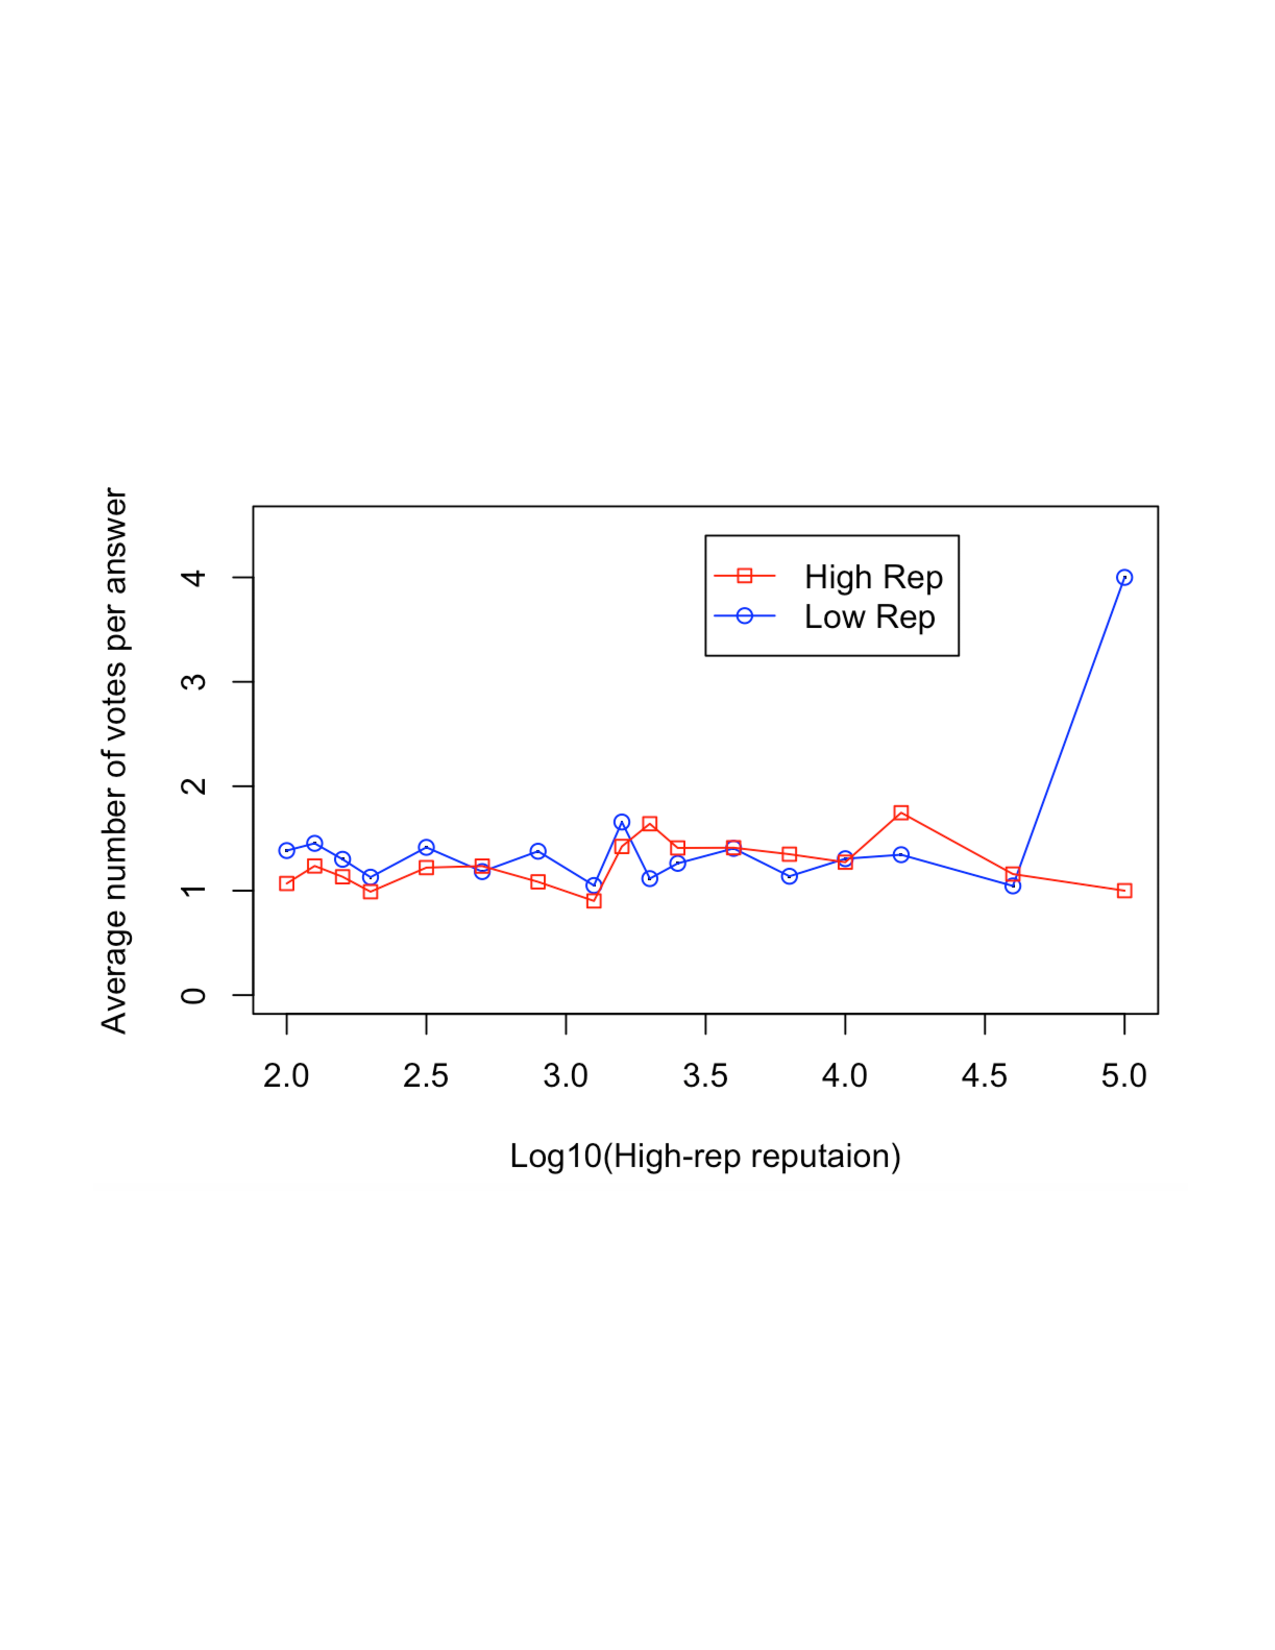
\includegraphics[width=0.8\columnwidth]{img/Fig6_2017.pdf}
    \caption{Average number of votes per answer for both answerers on a 2-answer question as a function of the higher answerer reputation. Lower reputation fixed between 75-125. High reputation plotted on a logarithmic (base 10) scale. (From 2015/07/31 to 2017/12/31)}
    \label{fig:fig6_2017}
\end{figure}

In order to answer the question above, we choose all the questions with exactly two answers as our target dataset. Suppose $r_{i}$ is the reputation of the \textit{i}-th answerer, and $v_{i}$ is the number of vote score of the \textit{i}-th answer. If there exists a trend where $v_{1}$ goes up while $v_{2}$ decreases, we consider there's a competitive relationship between two answerers. Now we set the value of $r_{i}$ unchanged as the x-axis, and compare the average vote score for both answerers. To begin with, we collected data from all questions with two answers, and separate answers according to answerers' reputation. Since the dataset is highly biased, majority users have very limited reputation, which means they are either non-active users or possibly non-questioner or answerer. Adopting data from this part of users can deviate our result, we set a threshold where lower reputation users of the two answerers should have reputation between 75 and 125. In order to make the graph easier to interpret, first we scale x-axis, which represents higher reputation users' reputation, using a logarithmic(base 10). For each reputation score, we use an average value to present higher and lower answerers' reputation respectively. Instead of representing vote score for each reputation point, we smooth the curve by splitting the vote scores into groups, according to different reputations in the x-axis, and calculate the average value of the group. From Fig\ref{fig:fig6_2010} we notice that in most cases, answer vote scores from high and low reputation users have a similar trend, they either decrease or increase together, but high reputation answerers' answer votes have higher variance. The corresponding pattern reveals that in most cases, the two answerers do not have a competitive relationship. Similarly, this trend can also be noticed during 2015 to 2017. However, we notice the later dataset have relatively less average vote score, this could probably indicate that although there are a great amount of newly introduced answers, the quality of such answers are not as good as before, or the question has been sufficiently answered, newly added answers does not contribute much to the question. 


%Fig7
\begin{figure}[!t]
    \centering
    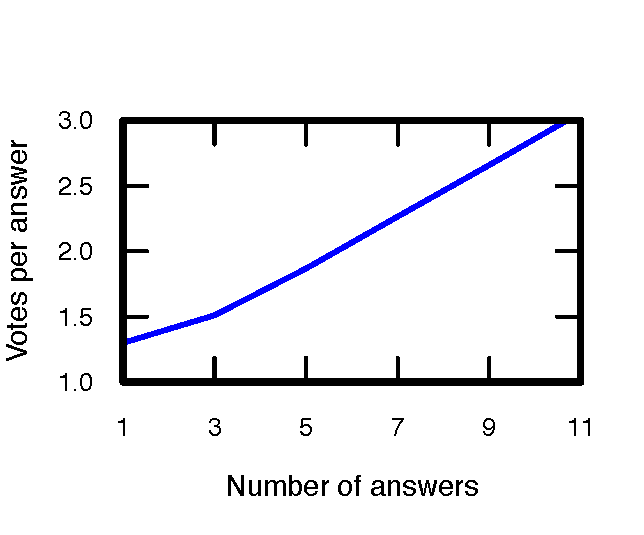
\includegraphics[width=0.8\columnwidth]{img/Fig7_2010.pdf}
    \caption{Number of votes per answer as a function of the number of answers on the question. (From 2008/07/31 to 2010/12/31)}
    \label{fig:fig7_2010}
\end{figure}

\begin{figure}[!t]
    \centering
    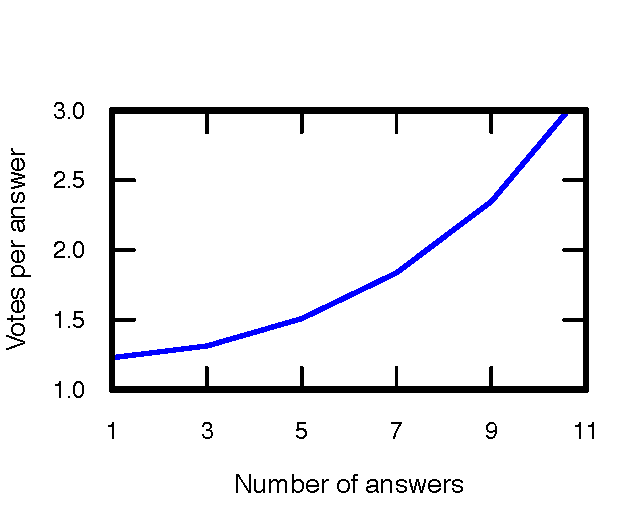
\includegraphics[width=0.8\columnwidth]{img/Fig7_2017.pdf}
    \caption{Number of votes per answer as a function of the number of answers on the question. (From 2015/07/31 to 2017/12/31)}
    \label{fig:fig7_2017}
\end{figure}
In the following step, we aim to investigate the relationship between the number of answers in each question, to the number of votes per answer. This work is to testify the correctness of the competition theory. If there exists a competitive relationship among answers, we would expect a decreasing number of votes per answer, as the number of answers increases. From Fig \ref{fig:fig7_2010} we find that from 2008 to 2010, the average number of votes display an ascending trend as the number of answers increases. This fact shows that the hotspot questions (questions with more answers) are more likely to benefit from community attention. Correspondingly, we also notice in Fig \ref{fig:fig7_2017}, where data is collected from 2015 to 2017, we find a similar upward trend for votes per answer as a function of the number of answers. From both of the two datasets we notice that, instead of competing for votes, all answers get more profit from communities involvement, especially for hotspot questions. 

%Fig8
\begin{figure}[!t]
    \centering
    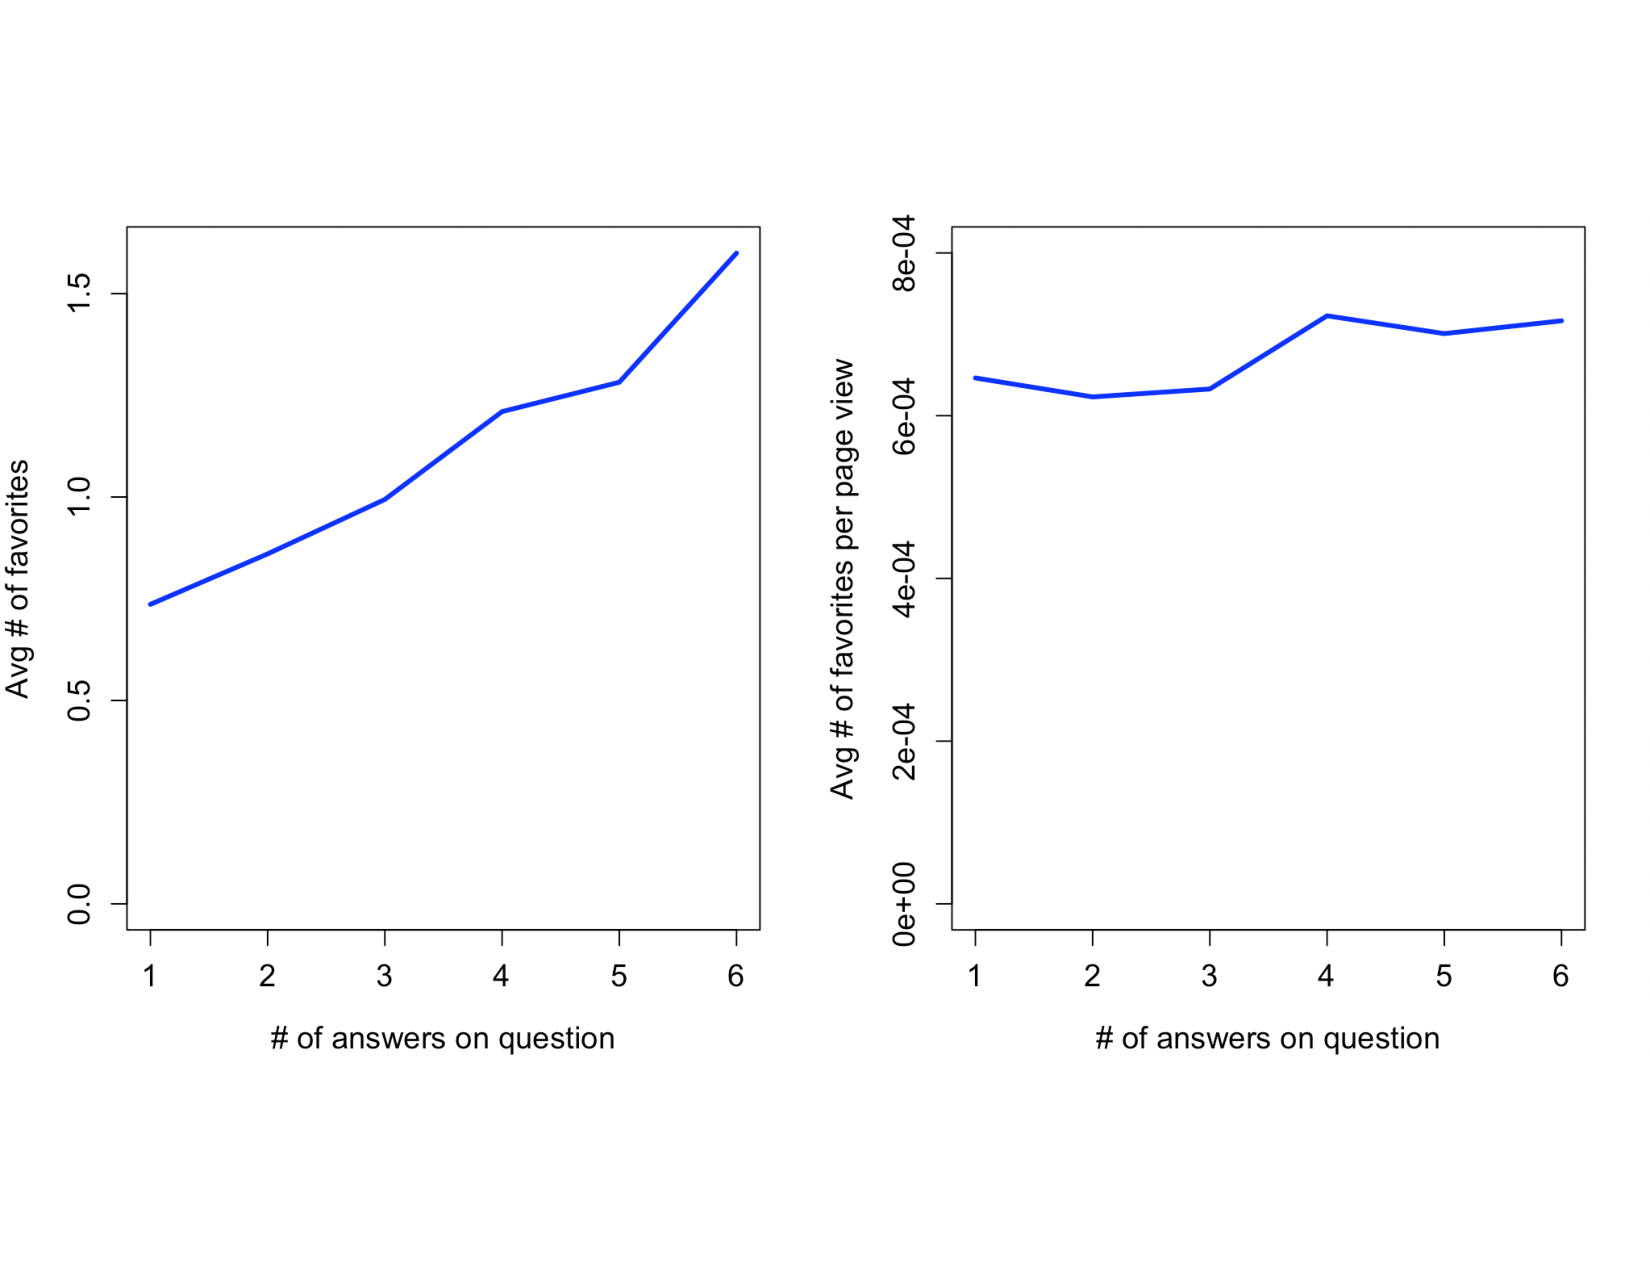
\includegraphics[width=\columnwidth]{img/Fig8_2010.pdf}
    \caption{(Left) Number of question favorites plotted against the number of answers over all questions where the maxi- mum answer vote score is 5. (Right) Same plot normalized by pageviews. (From 2008/07/31 to 2010/12/31)}
    \label{fig:fig8_2010}
\end{figure}

\begin{figure}[!t]
    \centering
    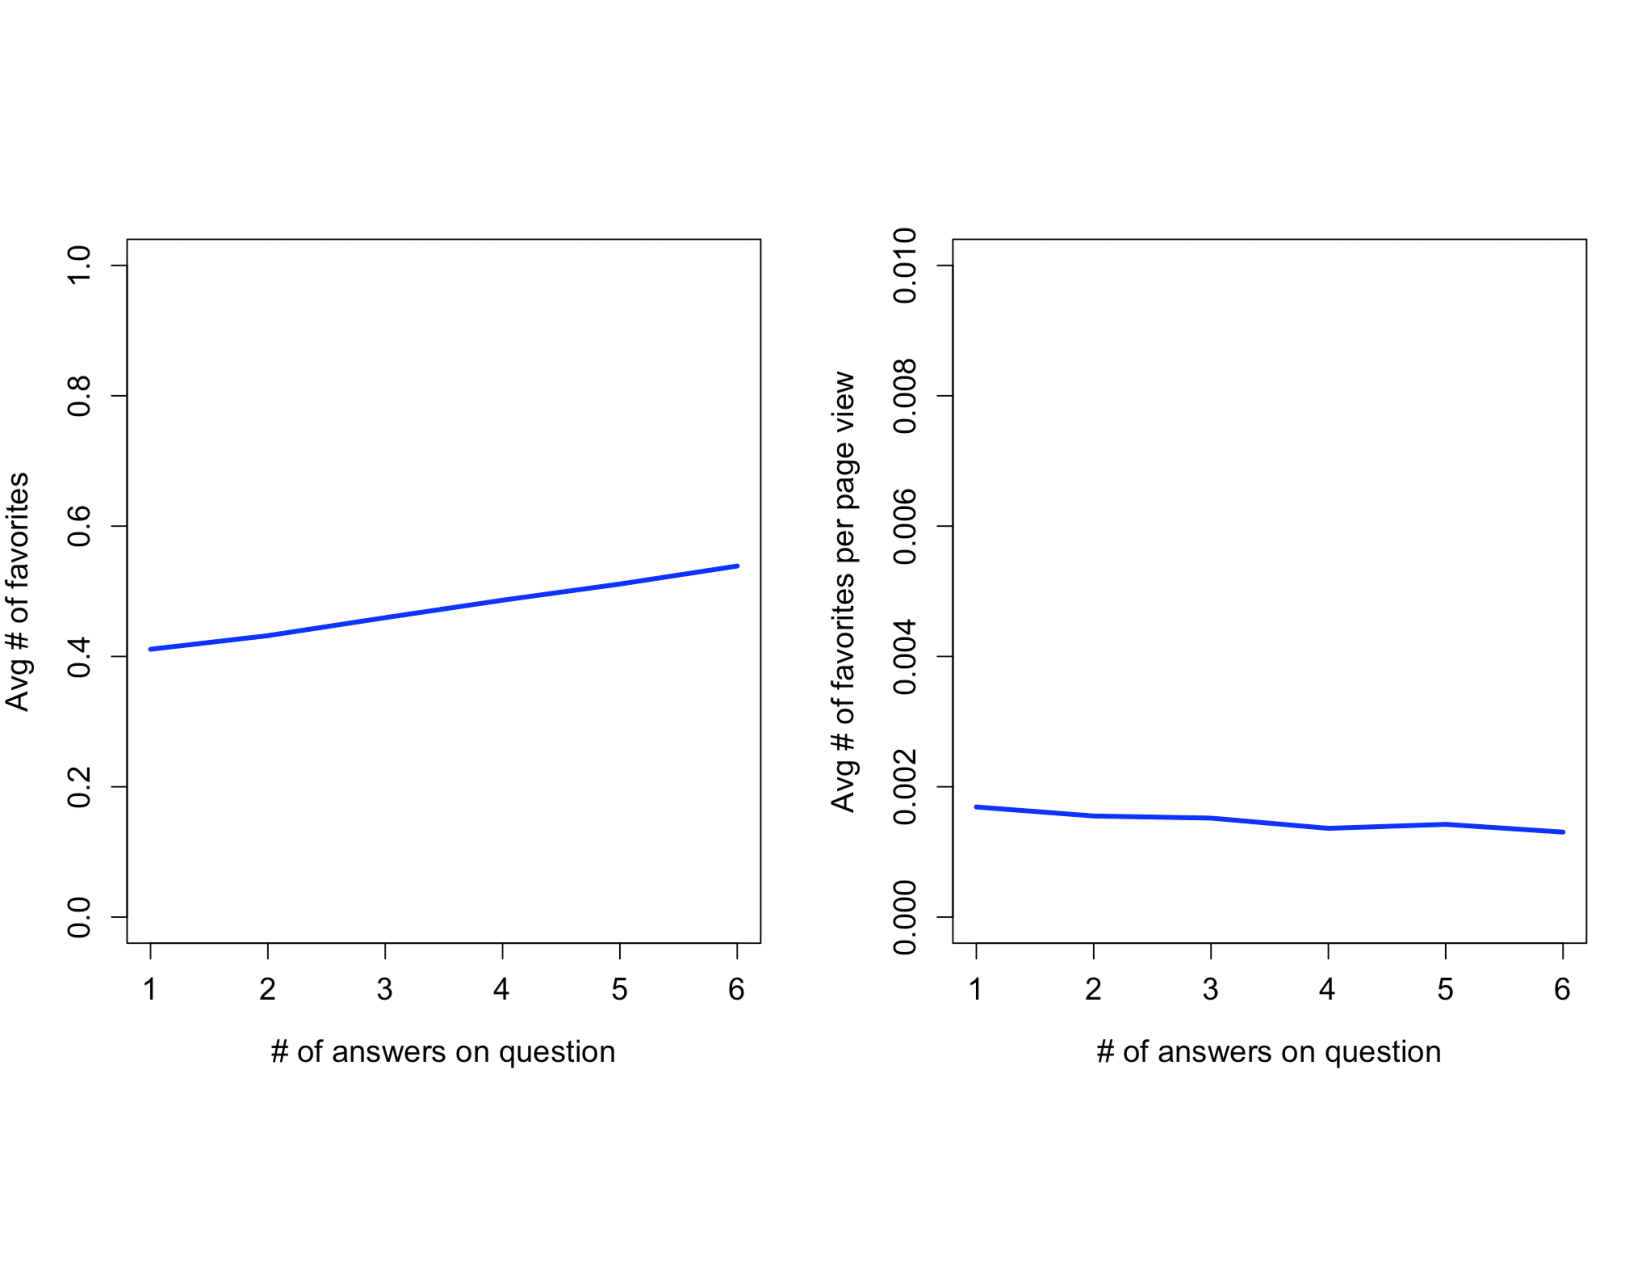
\includegraphics[width=\columnwidth]{img/Fig8_2017.pdf}
    \caption{(Left) Number of question favorites plotted against the number of answers over all questions where the maxi- mum answer vote score is 5. (Right) Same plot normalized by pageviews. (From 2015/07/31 to 2017/12/31)}
    \label{fig:fig8_2017}
\end{figure}

Apart from voting volcanism as an important source for evaluating community attention, favoring is also another channel to assess the quality of a question. In this part, our concern is whether questions with more answers receive more favorites from the community. In other words, we expect a hotspot question inclines to show its value by gaining more favorites. From previous study \cite{anderson2012discovering}, Anderson et al. found that among the highest voted answers of all questions, the highest voting score usually receives five votes. In this case, we first narrow our scope to the data from 2008 to 2010, to find all questions with the maximum answer vote score exactly equals to 5. From Fig \ref{fig:fig8_2010} we can find that the average number of favorites to a question is positively correlated to the number of answers in that question. As a question gaining more answers from community activities, it is probably because the same question is also shared by a wide range of groups. If there is an existing question proposed a commonly possessed confusion, answerers will get more votes for sharing their own experience and solution, and the question will be favored if users are satisfied to acquire instant solutions. 

Although we illustrate hotspot questions are more likely to gain a higher number of favorites, the favoriting process usually takes a relatively long time, after a question is posted and even sufficiently answered. During this time period, the potential answerers or users have same concerns will visit those QA pages, this will lead to a significant number accumulation in each question's favorite number. In order to avoid the interference from the number of page views, we normalize the data by dividing the number of favorites from the previous step by the number of page views. From Fig \ref{fig:fig8_2010} we find the average number of favorites per page view number is quite stable, which means users do not have a significant favoring preference on hotspot questions. 

Then we choose questions proposed between 2015 and 2017, where all the data are collected right after the end of 2017, this should reduce the error caused by analyzing questions with more than two years' favorites accumulation. From Fig \ref{fig:fig8_2017} we notice, even though the trend is similar as we illustrate before. However, we notice a significant scale change between those two figures. From 2015 to 2017, compared with the earlier dataset, we notice a significant decrease in the average number of favorites for all the questions. What's more, we also find the average number of favorites per page view has increased in these years. From our perspective, since we only study the questions posted in recent two years, those questions have relative low favorites number and page views. We think it is because Stack Overflow is already a mature knowledge sharing community after around ten years of development, most of the commonly possessed questions have been sufficiently answered. The newly introduced questions are either duplicating with previous questions or orienting a specific context and requiring expertise in that distinct domain. The duplicated questions will be marked and merged with previously proposed questions, and expertise questions are not accessible to the majority of community users cause they are targeting a special usage scenario. 

In this section, we can conclude that answers are not competing with others, all the answers will profit from continuous community involvement. Also, for hotspot questions with many answers, the more answer it gets, the more possible that both questions and their corresponding answers will receive more benefits.